\clearpage
\chapter{Study Guide 7}

\section{Matrices}
\horizontalline{0}{0}

\begin{center}
    \large{\textbf{Study Guide Instructions}}
\end{center}

\horizontalline{-1}{0}

\begin{itemize}
    \item Submit your work in Gradescope as a PDF - you will identify where your “questions are.”
    \item Identify the question number as you submit.  Since we grade "blind" if the questions are NOT identified, the work WILL NOT BE GRADED and a 0 will be recorded. Always leave enough time to 
    identify the questions when submitting.
    \item One section per page (if a page or less) - We prefer to grade the main solution in a single page, extra work can be included on the following page.
    \item Long instructions may be removed to fit on a single page.
    \item \textbf{Do not start a new question in the middle of a page.}
    \item Solutions to book questions are provided for reference.
    \item You may NOT submit given solutions - this includes minor modifications - as your own.
    \item Solutions that do not show individual engagement with the solutions will be marked as no credit and can be considered a violation of honor code.
    \item If you use the given solutions you must reference or explain how you used them, in particular...
\end{itemize}

\horizontalline{-1}{0}

\begin{center}
    \large{\textbf{Method Selection}}
\end{center}

\horizontalline{-1}{0}

\textbf{For full credit,  EACH book exercise in the Study Guides must use one or more of the following methods and FOR EACH QUESTION.  Identify the number the method by number to ensure full credit.}

\begin{itemize}
    \item \textbf{Method 1} - Provide original examples which demonstrate the ideas of the exercise in addition to your solution.
    \item \textbf{Method 2} - Include and discuss the specific topics needed from the chapter and how they relate to the question.
    \item \textbf{Method 3} - Include original Python code, of reasonable length (as screenshot or text)  to show how the topic or concept was explored.
    \item \textbf{Method 4} - Expand the given solution in a significant way, with additional steps and comments. All steps are justified. This is a good method for a proof for which you are only given a basic outline.
    \item \textbf{Method 5} - Attempt the exercise without looking at the solution and then the solution is used to check work. Words are used to describe the results.
    \item \textbf{Method 6} - Provide an analysis of the strategies used to understand the exercise, describing in detail what was challenging, who helped you or what resources were used. The process of understanding is
    described.
\end{itemize}

% Problem 1
\begin{problem}{Problem 1}
    \begin{statement}{Problem Statement}
        Annotate, summarize, and/or discuss the book example 7.4 Convolution. Be able to explain the basic ideas behind “blurring an image.” Which could be an exam question.
    \end{statement}

    \begin{Highlight}[Solution]
        For this annotation I am going to walk through a simple calculation of the element in the convolution matrix and discuss briefly what the values in the convolution matrix correspond to. \vspace*{1em}

        When calculating the convolution of a matrix, we use the following formula for a 2D convolution

        \setcounter{equation}{0}
        \begin{equation}
            C_{rs} = \sum_{i + k = r + 1, j + l = s + 1} A_{ij}B_{kl}, \hspace*{5pt} r = 1, \dots, m + p - 1, \hspace*{5pt} s = 1, \dots, n + q - 1.
        \end{equation}
        In (1), the original matrix $A$ is of the dimension $(m \times n)$ and the kernel matrix $B$ is of the dimension $(p \times q)$. The resulting convolution matrix is going to be of the dimension 
        $(m + p - 1) \times (n + q - 1)$. The original matrix $X$ that represents the image that is being blurred is

        \begin{equation}
            X = 
            \begin{bmatrix}
                1 & 1 & 1 & 1 & 1 & 1 & 1 & 1 & 1 \\
                1 & 1 & 1 & 1 & 1 & 1 & 1 & 1 & 1 \\
                1 & 1 & 0 & 0 & 0 & 0 & 0 & 1 & 1 \\
                1 & 1 & 1 & 0 & 1 & 1 & 0 & 1 & 1 \\
                1 & 1 & 1 & 0 & 1 & 1 & 0 & 1 & 1 \\
                1 & 1 & 1 & 0 & 1 & 1 & 0 & 1 & 1 \\
                1 & 1 & 1 & 1 & 1 & 1 & 1 & 1 & 1 \\
                1 & 1 & 1 & 1 & 1 & 1 & 1 & 1 & 1 \\
            \end{bmatrix}
        \end{equation}
        which is of the dimension $(m = 8) \times (n = 9)$. The kernel (or blurring matrix) is 

        \begin{equation}
            B = 
            \begin{bmatrix}
                1/4 & 1/4 \\
                1/4 & 1/4 \\
            \end{bmatrix}
        \end{equation}
        which is of the dimension $(p = 2) \times (q = 2)$. With this in mind this means that the convolution matrix $Y$ is going to be of the dimension $(8 + 2 - 1 = 9) \times (9 + 2 - 1 = 10)$.

        We can rewrite (1) to be in a more interpretable form as 

        \begin{equation}
            C_{rs} = \sum_{i = 1}^{m}\sum_{j = 1}^{n}\sum_{k = 1}^{p}\sum_{l = 1}^{q} A_{ij}B_{kl} \times \delta(i + k, r + 1) \times \delta(j + l, s + 1).
        \end{equation}
        In (4) the delta function acts as follows

        \begin{equation}
            \delta(\alpha,\beta) = \left\{
                \begin{aligned}
                    1 & & \text{If $\alpha = \beta$} \\
                    0 & & \text{Otherwise}
                \end{aligned}
            \right. .
        \end{equation}
        With this in mind, lets try to calculate $Y_{11}$. In this case $r = 1$ and $s = 1$. We begin the calculation
        \begin{align}
            Y_{11} & = \sum_{i = 1}^{8}\sum_{j = 1}^{9}\sum_{k = 1}^{2}\sum_{l = 1}^{2} A_{ij}B_{kl} \times \delta(i + k, 2) \times \delta(j + l, 2) \\
            & = \sum_{i = 1}^{8}\sum_{j = 1}^{9}\sum_{k = 1}^{2}\sum_{l = 1}^{2} A_{11}B_{11} \times \delta(2, 2) \times \delta(2, 2) \\
            & = \sum_{i = 1}^{8}\sum_{j = 1}^{9}\sum_{k = 1}^{2}\sum_{l = 1}^{2} A_{11}B_{11} \times (1) \times (1) \\
            & = \sum_{i = 1}^{8}\sum_{j = 1}^{9}\sum_{k = 1}^{2}\sum_{l = 1}^{2} (1)(1/4) = (1/4) \\
            & = (1/4) + \sum_{i = 1}^{8}\sum_{j = 1}^{9}\sum_{k = 1}^{2}\sum_{l = 1}^{2} A_{11}B_{12} \times \delta(2, 2) \times \delta(3, 2) \\
            & = (1/4) + \sum_{i = 1}^{8}\sum_{j = 1}^{9}\sum_{k = 1}^{2}\sum_{l = 1}^{2} A_{11}B_{12} \times (1) \times (0) \\
            & = (1/4) + 0 + \sum_{i = 1}^{8}\sum_{j = 1}^{9}\sum_{k = 1}^{2}\sum_{l = 1}^{2} A_{11}B_{21} \times \delta(3, 2) \times \delta(2, 2) \\
            & = (1/4) + 0 + \sum_{i = 1}^{8}\sum_{j = 1}^{9}\sum_{k = 1}^{2}\sum_{l = 1}^{2} A_{11}B_{21} \times (0) \times (1) \\
            & = (1/4) + 0 + \dots + 0 = (1/4).
        \end{align}
        Due to delta function in equation (6), the rest of the sums for $Y_{11}$ will be 0 and therefore $Y_{11} = (1/4)$. This result can be extrapolated for the rest of the values in $Y$ and when that
        is done we get the following matrix as the final result after the image blurring

        \begin{equation}
            Y = 
            \begin{bmatrix}
                1/4 & 1/2 & 1/2 & 1/2 & 1/2 & 1/2 & 1/2 & 1/2 & 1/2 & 1/4 \\
                1/2 & 1 & 1 & 1 & 1 & 1 & 1 & 1 & 1 & 1/2 \\
                1/2 & 1 & 3/4 & 1/2 & 1/2 & 1/2 & 1/2 & 3/4 & 1 & 1/2 \\
                1/2 & 1 & 3/4 & 1/4 & 1/4 & 1/2 & 1/4 & 1/2 & 1 & 1/2 \\
                1/2 & 1 & 1 & 1/2 & 1/2 & 1 & 1/2 & 1/2 & 1 & 1/2 \\
                1/2 & 1 & 1 & 1/2 & 1/2 & 1 & 1/2 & 1/2 & 1 & 1/2 \\
                1/2 & 1 & 1 & 3/4 & 3/4 & 1 & 3/4 & 3/4 & 1 & 1/2 \\
                1/2 & 1 & 1 & 1 & 1 & 1 & 1 & 1 & 1 & 1/2 \\
                1/4 & 1/2 & 1/2 & 1/2 & 1/2 & 1/2 & 1/2 & 1/2 & 1/2 & 1/4 \\
            \end{bmatrix}.
        \end{equation}
        The elements in $Y$ correspond to grey levels in the image. When this is applied the image blurring looks something like the following.

        \begin{center}
            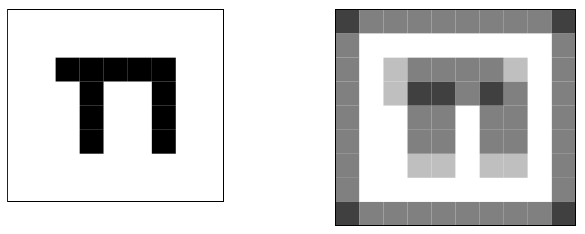
\includegraphics[width = 0.5\textwidth]{Images/Gray Levels.png}
        \end{center}
        The image on the left indicates the original image and the image on the left indicates the blurred image.
    \end{Highlight}
\end{problem}

% Problem 1 Summary
\begin{summary}{Problem 1 Summary}
    \begin{statement}{Procedure}
        \begin{itemize}
            \item Use the definition of convolution to calculate the convoluded matrix for the original matrix $X$ which represents the image that is being blurred.
        \end{itemize}
    \end{statement}
    \begin{statement}{Key Concepts}
        \begin{itemize}
            \item \textbf{Convolution in Image Processing:}
            \begin{itemize}
                \item The problem focuses on the concept of convolution, particularly in the context of image blurring.
                \item Convolution is a fundamental operation in image processing, used to modify images by applying filters (kernels).
            \end{itemize}
            \item \textbf{Matrix Representation of Images:}
            \begin{itemize}
                \item An image is represented as a matrix $X$, where each element corresponds to a pixel's intensity.
            \end{itemize}
            \item \textbf{Kernel or Blurring Matrix:}
            \begin{itemize}
                \item The kernel (or blurring matrix) $B$ is a smaller matrix used to blur the image.
                \item It's applied to each pixel and its neighbors to compute the blurred effect.
            \end{itemize}
            \item \textbf{Convolution Formula:}
            \begin{itemize}
                \item The convolution of an image matrix $X$ with a kernel $B$ is computed using a specific formula.
                \item The resulting convolution matrix $Y$ has dimensions determined by the sizes of $X$ and $B$.
            \end{itemize}
            \item \textbf{Calculation of Convolution Matrix:}
            \begin{itemize}
                \item The convolution matrix $Y$ is calculated element-wise, where each element corresponds to a weighted sum of pixel intensities, the weights being defined by the kernel $B$.
                \item This process simulates the blurring effect by averaging pixel values with their neighbors.
            \end{itemize}
            \item \textbf{Delta Function in Convolution:}
            \begin{itemize}
                \item A delta function is used in the convolution formula to handle boundary conditions and ensure that the computation only involves valid pixel locations.
            \end{itemize}
            \item \textbf{Resulting Blurred Image:}
            \begin{itemize}
                \item The elements in the convolution matrix $Y$ correspond to the grey levels in the blurred image.
                \item The final result demonstrates how the original image is blurred by the convolution process.
            \end{itemize}
        \end{itemize}
    \end{statement}
    \begin{statement}{Variations}
        \begin{itemize}
            \item We could be given a different image matrix to perform the convolution on.
            \begin{itemize}
                \item We would perform the same procedure on the new image with the kernel.
            \end{itemize}
        \end{itemize}
    \end{statement}
\end{summary}

% Problem 2
\begin{problem}{Problem 2}
    \begin{statement}{Problem Statement}
        Solve and explain the solution to 7.2  here in your own words. (Since you are given a solution, you will be graded on your ability to explain). \vspace*{1em}

        \noindent \textbf{Original Question:} \vspace*{1em}

        \textit{3-D rotation}. Let $x$ and $y$ be 3-vectors representing positions in 3-D. Suppose that the vector $y$ is obtained by rotating the vector $x$ about the vertical axis (i.e., $e_{3}$) 
        by $45^{\circ}$ (counterclockwise, i.e., from $e_{1}$ toward $e_{2}$). Find the $3 \times 3$ matrix $A$ for which $y = Ax$. \textit{Hint}. Determine the three columns of $A$ by finding the 
        result of the transformation on the unit vectors $e_{1}, e_{2}, e_{3}$.
    \end{statement}

    \begin{Highlight}[Solution]
        For this problem I will be using \textbf{Method 4}. \vspace*{1em}

        \noindent \textbf{VMLS Solution:} \vspace*{1em}
        
        \textbf{Solution}. We will construct A column by column. If we apply the given geometric transformation to $e_{1}$, we obtain the result ($1 / \sqrt{2}, 1 / \sqrt{2}, 0$). This is the first column of 
        $A$. When we apply the transformation to $e_{2}$, we get the result ($-1 / \sqrt{2}, 1 / \sqrt{2}, 0$), which is the second column of $A$. Finally, when we apply the transformation to $e_{3}$, 
        we simply get $e_{3} = (0,0,1)$, the third column of $A$. So we have

        \begin{equation*}
            A = 
            \begin{bmatrix}
                1 / \sqrt{2} & -1 / \sqrt{2} & 0 \\
                1 / \sqrt{2} & 1 / \sqrt{2} & 0 \\
                0 & 0 & 1 \\
            \end{bmatrix}.
        \end{equation*}

        \noindent \textbf{Explanation:} \vspace*{1em}

        For starters, if we wish to rotate a vector about the $z$ axis (this would be the $e_{3}$ unit vector) we need to use the standard rotation matrix in 3D for rotating about $z$. Namely,

        \setcounter{equation}{0}
        \begin{equation}
            R_{z}(\theta) = 
            \begin{bmatrix}
                \cos{(\theta)} & -\sin{(\theta)} & 0 \\
                \sin{(\theta)} & \cos{(\theta)} & 0 \\
                0 & 0 & 1 \\
            \end{bmatrix}.
        \end{equation}
        The problem statement requests that we rotate the vector $x$ by $45^{\circ}$ or $\frac{\pi}{4}$ radians. Consulting the unit circle, we know the unit values for cosine and sine at this angle are

        \begin{equation}
            \cos{\Big(\frac{\pi}{4}\Big)} = \sin{\Big(\frac{\pi}{4}\Big)} = \frac{1}{\sqrt{2}}.
        \end{equation}
        Using the result from equation (2) we know that our rotation matrix $A$ is then

        \begin{equation}
            A = 
            \begin{bmatrix}
                \cos{\Big(\frac{\pi}{4}\Big)} & -\sin{\Big(\frac{\pi}{4}\Big)} & 0 \\
                \sin{\Big(\frac{\pi}{4}\Big)} & \cos{\Big(\frac{\pi}{4}\Big)} & 0 \\
                0 & 0 & 1 \\
            \end{bmatrix}
            = 
            \begin{bmatrix}
                1 / \sqrt{2} & -1 / \sqrt{2} & 0 \\
                1 / \sqrt{2} & 1 / \sqrt{2} & 0 \\
                0 & 0 & 1 \\
            \end{bmatrix}.
        \end{equation}
        The result from equation (3) will in turn rotate a vector by $45^{\circ}$ about the $z$ axis.
    \end{Highlight}
\end{problem}

% Problem 2 Summary
\begin{summary}{Problem 2 Summary}
    \begin{statement}{Procedure}
        \begin{itemize}
            \item Use the rotation matrix around $z$ and plug in the values for $\theta$.
        \end{itemize}
    \end{statement}
    \begin{statement}{Key Concepts}
        \begin{itemize}
            \item \textbf{3D Rotation:}
            \begin{itemize}
                \item The problem focuses on rotating a vector in 3D space about a specific axis. It specifically looks at the rotation of a 3-vector $x$ to another 3-vector $y$ by rotating $x$ about 
                the vertical axis (denoted as $e_{3}$) by 45 degrees counterclockwise.
            \end{itemize}
            \item \textbf{Constructing Rotation Matrix $A$:}
            \begin{itemize}
                \item The goal is to find a $3 \times 3$ rotation matrix $A$ such that $y = Ax$.
                \item The method involves determining the columns of $A$ by applying the rotation to the unit vectors $e_{1}, e_{2},$ and $e_{3}$.
            \end{itemize}
            \item \textbf{Transformation of Unit Vectors:}
            \begin{itemize}
                \item Application of the transformation to $e_{1}$ and $e_{2}$ yields the first two columns of matrix $A$. The transformation of $e_{3}$ results in itself, forming the third column of $A$.
            \end{itemize}
            \item \textbf{Matrix Representation:}
            \begin{itemize}
                \item The resulting matrix $A$ is explicitly constructed with each column representing the transformed unit vectors.
                \item The matrix $A$ is represented as:
                \begin{equation*}
                    \begin{bmatrix}
                        1 / \sqrt{2} & -1 / \sqrt{2} & 0 \\
                        1 / \sqrt{2} & 1 / \sqrt{2} & 0 \\
                        0 & 0 & 1 \\
                    \end{bmatrix}.
                \end{equation*}
            \end{itemize}
            \item \textbf{Use of Standard Rotation Matrix:}
            \begin{itemize}
                \item The solution involves using the standard 3D rotation matrix for rotation about the $z$-axis.
                \item The rotation matrix $R_{z}(\theta)$ is formulated based on the angle of rotation $\theta$, with cosines and sines of $\theta$ occupying specific positions in the matrix.
            \end{itemize}
            \item \textbf{Calculation of Cosine and Sine Values:}
            \begin{itemize}
                \item For a 45-degree rotation, the sine and cosine values are both $\frac{1}{\sqrt{2}}$.
                \item These values are plugged into the standard rotation matrix formula to construct $A$.
            \end{itemize}
        \end{itemize}
    \end{statement}
    \begin{statement}{Variations}
        \begin{itemize}
            \item We could be asked to rotate the matrix around a different axis.
            \begin{itemize}
                \item In this case we would apply the correct rotation matrix and angle for this new axis rotation.
            \end{itemize}
        \end{itemize}
    \end{statement}
\end{summary}

% Problem 3
\begin{problem}{Problem 3}
    \begin{statement}{Problem Statement}
        Solve and Explain the solution to 7.3  here in your own words. (Since you are given a solution, you will be graded on your ability to explain). \vspace*{1em}

        \noindent \textbf{Original Question:} \vspace*{1em}

        \textit{Trimming a vector}. Find a matrix $A$ for which $Ax = (x_{2}, \dots , x_{n - 1})$, where $x$ is an $n$-vector. (Be sure to specify the size of $A$, and describe all its entries.)
    \end{statement}

    \begin{Highlight}[Solution]
        For this problem I will be using \textbf{Method 4}. \vspace*{1em}

        \noindent \textbf{VMLS Solution:} \vspace*{1em}

        \textbf{Solution}. $A$ is an $(n - 2) \times n$ matrix with entries

        \begin{equation*}
            x = \left\{
                \begin{aligned}
                    1 & & i = j - 1 \\
                    0 & & \text{Otherwise} 
                \end{aligned}
            \right.
        \end{equation*}
        Written out in terms of its entries, we have

        \begin{equation*}
            A = 
            \begin{bmatrix}
                0 & 1 & 0 & 0 & \dots & 0 & 0 \\
                0 & 0 & 1 & 0 & \dots & 0 & 0 \\
                0 & 0 & 0 & 1 & \dots & 0 & 0 \\
                \vdots & \vdots & \vdots & \vdots & \ddots & \vdots & \vdots \\
                0 & 0 & 0 & 0 & \dots & 1 & 0 \\
            \end{bmatrix}
            = 
            \begin{bmatrix}
                0_{(n-2)\times 1} & I_{(n-2)} & 0_{(n - 2) \times 1}.
            \end{bmatrix}.
        \end{equation*}
        The subscripts in the last expression indicate the dimensions for clarity.

        We can justify this choice of $A$ several ways. Working by columns, we can ask what should $Ae_{1}$ be? The answer is 0. This is the first column of $A$. What is $Ae_{2}$? It is $e_{1}$, which 
        is the second column of $A$. And so on.

        We can also work with the rows. The first row of $A$ tells us how to get $(Ax)_{1}$. This should by choosing $x_{2}$, which means the first row is $e^{T}_{2}$. And so on. \vspace*{1em}

        \noindent \textbf{Explanation:} \vspace*{1em}

        The problem statement is asking us to construct a matrix that has one entry for every row. Particularly, a 1 for every row and the rest of the entries in that row must be zero. The first row is
        to have the vector $(x_{2})$ in it, which means the trailing entry in that row must be a 0.

        Lets say that $n=4$ just for an example. This means the resulting vector would need to be $(x_{2},x_{3})$ after the matrix $A$ acts on $x$. For this to work, we would need to require that $A$ has
        the same number of columns as $x$ as rows. In our supposed example, this would mean that $A$ would have to have 4 rows since $x$ has four columns ($n = 4$ in this example). Namely,

        \setcounter{equation}{0}
        \begin{equation}
            Ax = 
            \begin{bmatrix}
                0 & 1 & 0 & 0 \\
                0 & 0 & 1 & 0 \\
            \end{bmatrix}
            \begin{bmatrix}
                x_{1} \\
                x_{2} \\
                x_{3} \\
                x_{4} \\
            \end{bmatrix}
            = 
            \begin{bmatrix}
                x_{2} \\
                x_{3} \\
            \end{bmatrix}.
        \end{equation}
        From the result in equation (1) we can see that $A$ has two less rows than it does columns. So in general the dimension of $A$ is then

        \begin{equation}
            A_{(n - 2) \times n}.
        \end{equation}
        If we examine closely, we can see that $A$ has the identity matrix sandwiched in between the outer columns of it. So, if we wish to extrapolate on this further we could generalize $A$ to be

        \begin{equation}
            A = 
            \begin{bmatrix}
                0 & 1 & 0 & 0 & \dots & 0 & 0 \\
                0 & 0 & 1 & 0 & \dots & 0 & 0 \\
                0 & 0 & 0 & 1 & \dots & 0 & 0 \\
                \vdots & \vdots & \vdots & \vdots & \ddots & \vdots & \vdots \\
                0 & 0 & 0 & 0 & \dots & 1 & 0 \\
            \end{bmatrix}.
        \end{equation}
        To represent (3) in a block matrix we could succinctly write it as 

        \begin{equation}
            A =
            \begin{bmatrix}
                0_{(n-2)\times 1} & I_{(n-2)} & 0_{(n - 2) \times 1}.
            \end{bmatrix}
        \end{equation}
        Where in English, the first and last columns of $A$ are the 0 vector of $(n - 2) \times 1$ size and the middle columns are the identity matrix of $(n - 2)$ size. The entries of $A$ are then
        described as 

        \begin{equation}
            x = \left\{
                \begin{aligned}
                    1 & & i = j - 1 \\
                    0 & & \text{Otherwise} 
                \end{aligned}
            \right.
        \end{equation}
        where we get a 1 as the entry if $i^{\text{th}}$ row is one less than the $j^{\text{th}}$ column. Otherwise the entries are 0.
    \end{Highlight}
\end{problem}

% Problem 3 Summary
\begin{summary}{Problem 3 Summary}
    \begin{statement}{Procedure}
        \begin{itemize}
            \item Create a simple matrix where the resulting matrix is of $2 \times 1$.
            \item Extrapolate on the previous simple example to create the matrix that is desired of us.
            \item Write the new matrix in a block matrix form.
        \end{itemize}
    \end{statement}
    \begin{statement}{Key Concepts}
        \begin{itemize}
            \item \textbf{Problem Statement:}
            \begin{itemize}
                \item The task is to find a matrix $A$ such that for an $n$-vector $x$, the product $Ax$ results in a vector where the first component of $x$ is removed, 
                effectively 'trimming' the vector.
                \item The matrix $A$ needs to be defined in terms of its size and the nature of its entries.
            \end{itemize}
            \item \textbf{Solution Approach:}
            \begin{itemize}
                \item The solution involves defining $A$ as an $(n-2) \times n$ matrix.
                \item The entries of $A$ are constructed such that when multiplied with $x$, the resulting vector is $x$ with its first element removed.
                \item The matrix $A$ is structured to have its diagonal elements (excluding the first row) set to 1 and all other elements set to 0.
            \end{itemize}
            \item \textbf{Matrix Structure:}
            \begin{itemize}
                \item The matrix $A$ is characterized by having zero entries in its first row and column, and an identity matrix of size $(n-2)$ in its lower-right block.
                \item It can be represented in a block matrix form as:
                \begin{equation*}
                    A = 
                    \begin{bmatrix} 
                        0_{(n-2) \times 1} & I_{(n-2)} & 0_{(n-2) \times 1} 
                    \end{bmatrix}
                \end{equation*}
                \item The notation $0_{(n-2) \times 1}$ represents a column of zeros with $n-2$ entries, and $I_{(n-2)}$ is the identity matrix of size $(n-2)$.
            \end{itemize}
            \item \textbf{Linear Algebra Concepts:}
            \begin{itemize}
                \item The problem exemplifies the use of matrix operations to transform vectors.
                \item It demonstrates how the structure of a matrix can be tailored to achieve a specific vector transformation.
            \end{itemize}
        \end{itemize}
    \end{statement}
    \begin{statement}{Variations}
        \begin{itemize}
            \item We could be given a different desired result for the `trimmed' vector.
            \begin{itemize}
                \item In this case we would use the same logic, try a simple example first, and then extrapolate to form a matrix that achieves of this result.
            \end{itemize}
        \end{itemize}
    \end{statement}
\end{summary}

% Problem 4
\begin{problem}{Problem 4}
    \begin{statement}{Problem Statement}
        Solve and Explain the solution to 7.7 here in your own words. (Since you are given a solution, you will be graded on your ability to explain). \vspace*{1em}

        \noindent \textbf{Original Question:} \vspace*{1em}

        \textit{Incidence matrix of reversed graph}. (See exercise 6.5.) Suppose $A$ is the incidence matrix of a graph. The reversed graph is obtained by reversing the directions of all the edges of the 
        original graph. What is the incidence matrix of the reversed graph? (Express your answer in terms of $A$.)
    \end{statement}

    \begin{Highlight}[Solution]
        For this problem I will be using \textbf{Method 4}. \vspace*{1em}

        \noindent \textbf{VMLS Solution:} \vspace*{1em}

        \textbf{Solution}. $-A$. \vspace*{1em}

        \noindent \textbf{Explanation:} \vspace*{1em}

        According to the notion of direction described by the author of VMLS, the direction of edges in an incidence matrix are described as

        \begin{equation*}
            A_{ij} = \left\{
                \begin{aligned}
                    1 & & \text{Edge $j$ points to node $i$} \\
                    -1 & & \text{Edge $j$ points from node $i$} \\
                    0 & & \text{Otherwise}
                \end{aligned}
            \right. .
        \end{equation*}
        In English, if an edge points away from a node it is indicated with the value of -1. If an edge points into a node it is indicated with with the value of 1.

        If we wish to reverse the direction of edges, we need to change the -1's to 1's and the 1's to -1's. So, mathematically we need to multiply the incidence matrix $A$ by -1. Namely,

        \setcounter{equation}{0}
        \begin{equation}
            -A.
        \end{equation}
        Equation (1) represents how we would reverse the direction of a graph with the use of an incidence matrix.
    \end{Highlight}
\end{problem}

% Problem 4 Summary
\begin{summary}{Problem 4 Summary}
    \begin{statement}{Procedure}
        \begin{itemize}
            \item Define what the direction of edges mean in regards to signs in a graph.
            \item Translate this into an incidence matrix.
            \item Show that multiplying by -1 produces a reversed graph.
        \end{itemize}
    \end{statement}
    \begin{statement}{Key Concepts}
        \begin{itemize}
            \item \textbf{Problem Statement:}
            \begin{itemize}
                \item Given an incidence matrix $A$ of a graph, the objective is to determine the incidence matrix of the reversed graph.
                \item The reversed graph is obtained by reversing the directions of all edges in the original graph.
            \end{itemize}
            \item \textbf{Solution:}
            \begin{itemize}
                \item The solution to the problem is given by the expression $-A$.
                \item Reversing the direction of each edge in the graph corresponds to changing the sign of each non-zero entry in the incidence matrix $A$.
            \end{itemize}
            \item \textbf{Explanation:}
            \begin{itemize}
                \item In an incidence matrix:
                \begin{itemize}
                    \item An entry $A_{ij}$ is $-1$ if edge $j$ points away from node $i$.
                    \item An entry $A_{ij}$ is $1$ if edge $j$ points towards node $i$.
                \end{itemize}
                \item To reverse the direction of the edges, each $-1$ becomes $1$ and each $1$ becomes $-1$. This operation is equivalent to multiplying the incidence matrix $A$ 
                by $-1$.
            \end{itemize}
            \item \textbf{Mathematical Representation:}
            \begin{itemize}
                \item The incidence matrix of the reversed graph is represented mathematically as:
                \begin{equation*}
                    -A.
                \end{equation*}
                \item This operation effectively inverts the directionality encoded in the original incidence matrix.
            \end{itemize}
            \item \textbf{Significance in Linear Algebra}
            \begin{itemize}
                \item This problem demonstrates the application of matrix operations in graph theory.
                \item It highlights how simple transformations can represent significant changes in the structure of a graph.
            \end{itemize}
        \end{itemize}
    \end{statement}
    \begin{statement}{Variations}
        \begin{itemize}
            \item This problem does not really lend itself to be different, instead we could be asked to create an incidence matrix from a graph.
            \begin{itemize}
                \item In this case we would us the signs to determine the direction of edges in a graph that would be inserted into an incidence matrix.
            \end{itemize}
        \end{itemize}
    \end{statement}
\end{summary}

% Problem 5
\begin{problem}{Problem 5}
    \begin{statement}{Problem Statement}
        Solve and Explain the solution to 7.9 here in your own words. (Since you are given a solution, you will be graded on your ability to explain). \vspace*{1em}

        \noindent \textbf{Original Question:} \vspace*{1em}

        \textit{Social network graph}. Consider a group of $n$ people or users, and some symmetric social relation among them. This means that some pairs of users are connected, or friends (say). We can create 
        a directed graph by associating a node with each user, and an edge between each pair of friends, arbitrarily choosing the direction of the edge. Now consider an $n$-vector $v$, where $v_{i}$ 
        is some quantity for user $i$, for example, age or education level (say, given in years). Let $\mathcal{D}(v)$ denote the Dirichlet energy associated with the graph and $v$, thought of as a 
        potential on the nodes.

        \begin{enumerate}[label = (\alph*)]
            \item Explain why the number $\mathcal{D}(v)$ does not depend on the choice of directions for the edges of the graph.
            \item Would you guess that $\mathcal{D}(v)$ is small or large? This is an open-ended, vague question; there is no right answer. Just make a guess as to what you might expect, and give a 
            short English justification of your guess.
        \end{enumerate}
    \end{statement}

    \begin{Highlight}[Solution - Part (a)]
        For this problem I will be using \textbf{Method 4}. \vspace*{1em}

        \noindent \textbf{VMLS Solution:} 

        \begin{enumerate}[label = (\alph*)]
            \item The Dirichlet energy has the form
            
            \begin{equation*}
                \mathcal{D}(v) = \sum_{(i,j) \in \mathcal{E}} (v_{i} - v_{j})^{2},
            \end{equation*}
            where $\mathcal{E}$ is the set of edges of the graph, which correspond to pairs $(i, j)$ of individuals who are friends. If we switch the orientation of edge between $i$ and $j$, the term 
            $(v_{i} - v_{j})^{2}$ becomes $(v_{j} - v_{i})^{2}$, which is the same.
        \end{enumerate}

        \noindent \textbf{Explanation:}

        \begin{enumerate}[label = (\alph*)]
            \item We know from VMLS that the Dirichlet energy can be calculated with 
            
            \begin{equation*}
                \mathcal{D}(v) = \|A^{T}v\|^{2} = \sum_{\text{edges } (k,l)} (v_{l} - v_{k})^{2}.
            \end{equation*}
            In the context of our problem we can represent the Dirichlet energy as

            \setcounter{equation}{0}
            \begin{equation}
                \mathcal{D}(v) = \sum_{(i,j) \in \mathcal{E}} (v_{i} - v_{j})^{2}.
            \end{equation}
            In the context of equation (1) we are representing the edges in question with $\mathcal{E}$. Since the quantity $v_{i} - v_{j}$ is being squared in this calculation, the direction of the 
            edges will not affect the resulting calculation. So from this we can say that the orientation between $i$ and $j$ is not important. In short, $\mathbf{v_{i} - v_{j}} \textbf{ is being squared}$ 
            and therefore the orientation does not matter.
        \end{enumerate}
    \end{Highlight}

    \begin{Highlight}[Solution - Part (b)]
        For this problem I will be using \textbf{Method 4}. \vspace*{1em}

        \noindent \textbf{VMLS Solution:} 

        \begin{enumerate}[label = (\alph*), start = 2]
            \item You might guess that $\mathcal{D}(v)$ is small. This means that friends tend to have similar values of the quantity represented by $v$. For example, your circle of friends probably mostly 
            have ages similar to yours, education levels similar to yours, and so on.
        \end{enumerate}

        \noindent \textbf{Explanation:} 

        \begin{enumerate}[label = (\alph*), start = 2]
            \item In the Dirichlet energy calculation we are calculating the difference between the quantities $v$. Since we are working with a domain relative to us, we would most likely be working with quantities
            that are similar to ourself. If $v$ represents age, then it would be appropriate to believe that $\mathcal{D}(v)$ would be small. If $v$ were something else, it could range from being large to small.
            This is really dependent upon the person and the person that they are friends with.
        \end{enumerate}
    \end{Highlight}
\end{problem}

% Problem 5 Summary
\begin{summary}{Problem 5 Summary}
    \begin{statement}{Procedure}
        \begin{itemize}
            \item For part (a), reason that because of the squaring that occurs in the Dirichlet energy equation, the direction of the edges does not matter when calculating.
            \item For part (b), reason what the value would be in terms of magnitude for what the edges represent in the graph.
        \end{itemize}
    \end{statement}
    \begin{statement}{Key Concepts}
        \begin{itemize}
            \item \textbf{Problem Statement:}
            \begin{itemize}
                \item The problem considers a social network graph represented as a directed graph with nodes corresponding to individuals and edges to friendships.
                \item An $n$-vector $v$ represents a certain quantity associated with each individual, like age or education level.
                \item The focus is on the Dirichlet energy $D(v)$ associated with this graph and vector $v$.
            \end{itemize}
            \item \textbf{Dirichlet Energy:}
            \begin{itemize}
                \item The Dirichlet energy $D(v)$ is defined as the sum of squared differences between connected individuals' quantities:
                \begin{equation*}
                    D(v) = \sum_{(ij) \in E} (v_i - v_j)^2.
                \end{equation*}
                \item This sum extends over all edges $E$ in the graph.
            \end{itemize}
            \item \textbf{Independence of Edge Directions:}
            \begin{itemize}
                \item The problem explores why the value of $D(v)$ is independent of the orientation of the edges in the graph.
                \item The symmetry in the squared difference \((v_i - v_j)^2\) ensures that reversing the direction of an edge does not affect the Dirichlet energy.
            \end{itemize}
            \item \textbf{Magnitude of Dirichlet Energy:}
            \begin{itemize}
                \item A hypothesis is made about whether $D(v)$ is expected to be large or small in a typical social network.
                \item The reasoning is based on the assumption that friends (connected nodes) tend to have similar values for the quantities represented by $v$.
                \item It is guessed that $D(v)$ is likely small, indicating similarity in the quantities $v$ among friends.
            \end{itemize}
            \item \textbf{Linear Algebra Context}
            \begin{itemize}
                \item The problem leverages the concepts of graph theory and linear algebra to quantify relationships in a network.
                \item It demonstrates how linear algebra can be used to model and analyze real-world social network structures.
            \end{itemize}
        \end{itemize}
    \end{statement}
    \begin{statement}{Variations}
        \begin{itemize}
            \item We could be asked to determine the Dirichlet energy for a different graph.
            \begin{itemize}
                \item In this case we would use the same procedure of determining what the values would represent inside that graph.
            \end{itemize}
        \end{itemize}
    \end{statement}
\end{summary}

% Problem 6
\begin{problem}{Problem 6}
    \begin{statement}{Problem Statement}
        Solve and Explain the solution to 7.10 here in your own words. (Since you are given a solution, you will be graded on your ability to explain). \vspace*{1em}

        \noindent \textbf{Original Question:} \vspace*{1em}

        Circle graph. A circle graph (also called a cycle graph) has n vertices, with edges pointing from vertex 1 to vertex 2, from vertex 2 to vertex 3, $\dots$ , from vertex $n - 1$ to vertex $n$, and finally, from 
        vertex $n$ to vertex 1. (This last edge completes the circle.)

        \begin{enumerate}[label = (\alph*)]
            \item Draw a diagram of a circle graph, and give its incidence matrix $A$.
            \item Suppose that $x$ is a circulation for a circle graph. What can you say about $x$?
            \item Suppose the $n$-vector $v$ is a potential on a circle graph. What is the Dirichlet energy $\mathcal{D}(v) = \|A^{T}v\|^{2}$?
        \end{enumerate}
    \end{statement}

    \begin{Highlight}[Solution - Part (a)]
        For this problem I will be using \textbf{Method 4}. \vspace*{1em}

        \noindent \textbf{VMLS Solution:} 

        \begin{enumerate}[label = (\alph*)]
            \item The figure shows the circle graph with 6 nodes.
            \begin{center}
                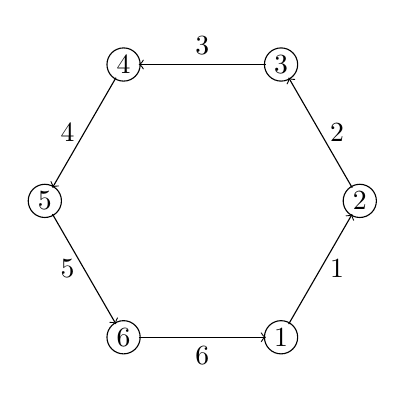
\begin{tikzpicture}
                    \coordinate (F) at (0,0);
                    \coordinate (A) at (2,0);
                    \coordinate (B) at (3,1.732);
                    \coordinate (C) at (2,3.464);
                    \coordinate (D) at (0,3.464);
                    \coordinate (E) at (-1,1.732);
                    
                    \foreach \point/\label in {A/1,B/2,C/3,D/4,E/5,F/6}
                        \node[circle, draw, inner sep=0pt, minimum size=12pt] (\label) at (\point) {\label};
                    
                    \draw[->, shorten >=5.5pt, shorten <=5.5pt] (A) -- node[midway, right] {1} (B);
                    \draw[->, shorten >=5.5pt, shorten <=5.5pt] (B) -- node[midway, right] {2} (C);
                    \draw[->, shorten >=5.5pt, shorten <=5.5pt] (C) -- node[midway, above] {3} (D);
                    \draw[->, shorten >=5.5pt, shorten <=5.5pt] (D) -- node[midway, left] {4} (E);
                    \draw[->, shorten >=5.5pt, shorten <=5.5pt] (E) -- node[midway, left] {5} (F);
                    \draw[->, shorten >=5.5pt, shorten <=5.5pt] (F) -- node[midway, below] {6} (A);
                \end{tikzpicture}
            \end{center}
            The incidence matrix is

            \begin{equation*}
                A = 
                \begin{bmatrix}
                    -1 & 0 & 0 & 0 & 0 & 1 \\
                    1 & -1 & 0 & 0 & 0 & 0 \\
                    0 & 1 & -1 & 0 & 0 & 0 \\
                    0 & 0 & 1 & -1 & 0 & 0 \\
                    0 & 0 & 0 & 1 & -1 & 0 \\
                    0 & 0 & 0 & 0 & 1 & -1 \\
                \end{bmatrix}
            \end{equation*}
        \end{enumerate}

        \textbf{Explanation:}

        \begin{enumerate}[label = (\alph*)]
            \item In the spirit of generating an example that is different from VMLS', this figure shows the cycle graph with 3 nodes
            
            \begin{center}
                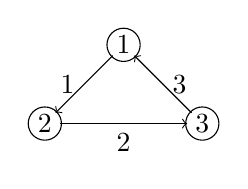
\begin{tikzpicture}
                    \coordinate (A) at (0,0);
                    \coordinate (B) at (-1,-1);
                    \coordinate (C) at (1,-1);
                    
                    \foreach \point/\label in {A/1,B/2,C/3}
                        \node[circle, draw, inner sep=0pt, minimum size=12pt] (\label) at (\point) {\label};
                    
                    \draw[->, shorten >=5.5pt, shorten <=5.5pt] (A) -- node[midway, left] {1} (B);
                    \draw[->, shorten >=5.5pt, shorten <=5.5pt] (B) -- node[midway, below] {2} (C);
                    \draw[->, shorten >=5.5pt, shorten <=5.5pt] (C) -- node[midway, right] {3} (A);
                \end{tikzpicture}
            \end{center}

            The incidence matrix of this is then

            \setcounter{equation}{0}
            \begin{equation}
                A = 
                \begin{bmatrix}
                    -1 & 0 & 1 \\
                    1 & -1 & 0 \\
                    0 & 1 & -1 \\
                \end{bmatrix}.
            \end{equation}
        \end{enumerate}
    \end{Highlight}

    \begin{Highlight}[Solution - Part (b)]
        For this problem I will be using \textbf{Method 4}. \vspace*{1em}

        \noindent \textbf{VMLS Solution:} 

        \begin{enumerate}[label = (\alph*), start = 2]
            \item The entries of $x$ are equal.
        \end{enumerate}

        \noindent \textbf{Explanation:}

        \begin{enumerate}[label = (\alph*), start = 2]
            \item In a cycle graph like the ones above, the number of edges that are leaving a node is equal to the number of edges that are incoming to a node. Because of this fact flow conservation
            occurs and we have the relationship

            \begin{equation}
                Ax = 0.
            \end{equation}
            Expanding (2) we have

            \begin{equation}
                Ax = 
                \begin{bmatrix}
                    -1 & 0 & 0 & 0 & 0 & 1 \\
                    1 & -1 & 0 & 0 & 0 & 0 \\
                    0 & 1 & -1 & 0 & 0 & 0 \\
                    0 & 0 & 1 & -1 & 0 & 0 \\
                    0 & 0 & 0 & 1 & -1 & 0 \\
                    0 & 0 & 0 & 0 & 1 & -1 \\
                \end{bmatrix}
                \begin{bmatrix}
                    x_{1} \\
                    x_{2} \\
                    x_{3} \\
                    x_{4} \\
                    x_{5} \\
                    x_{6} \\
                \end{bmatrix}
                = 
                \begin{bmatrix}
                    0 \\
                    0 \\
                    0 \\
                    0 \\
                    0 \\
                    0 \\
                \end{bmatrix}.
            \end{equation}
            Determining the values of $x_{i}$ involves solving a system of equations. When one solves this system of equations we find that the values of $x$ are all equal.
        \end{enumerate}
    \end{Highlight}

    \begin{Highlight}[Solution - Part (c)]
        For this problem I will be using \textbf{Method 4}. \vspace*{1em}

        \noindent \textbf{VMLS Solution:} 

        \begin{enumerate}[label = (\alph*), start = 3]
            \item $\mathcal{D}(v) = (v_{2} - v_{1})^{2} + (v_{3} - v_{2})^{2} + \dots + (v_{n} - v_{n - 1})^{2} + (v_{1} - v_{n})^{2}.$
        \end{enumerate}

        \noindent \textbf{Explanation:}

        \begin{enumerate}[label = (\alph*), start = 3]
            \item The formula for calculating the Dirichlet energy is 
            
            \begin{equation*}
                \mathcal{D}(v) = \|A^{T}v\|^{2} = \sum_{\text{edges } (k,l)} (v_{l} - v_{k})^{2}.
            \end{equation*}
            Applying this to the example that was given from the graph that was given by VMLS we see
            \setcounter{equation}{0}
            \begin{align}
                \text{Edge 1: } & l = 2, k = 1 & (v_{l} - v_{k})^{2} = (v_{2} - v_{1})^{2} \\
                \text{Edge 2: } & l = 3, k = 2 & (v_{l} - v_{k})^{2} = (v_{3} - v_{2})^{2} \\
                \text{Edge 3: } & l = 4, k = 3 & (v_{l} - v_{k})^{2} = (v_{4} - v_{3})^{2} \\
                \text{Edge 4: } & l = 5, k = 4 & (v_{l} - v_{k})^{2} = (v_{5} - v_{4})^{2} \\
                \text{Edge 5: } & l = 6, k = 5 & (v_{l} - v_{k})^{2} = (v_{6} - v_{5})^{2} \\
                \text{Edge 5: } & l = 1, k = 6 & (v_{l} - v_{k})^{2} = (v_{1} - v_{6})^{2}
            \end{align}
            Putting this together we then have
            \begin{equation}
                \mathcal{D}(v) = (v_{2} - v_{1})^{2} + (v_{3} - v_{2})^{2} + (v_{4} - v_{3})^{2} + (v_{5} - v_{4})^{2} + (v_{6} - v_{5})^{2} + (v_{1} - v_{6})^{2}.
            \end{equation}
        \end{enumerate}
    \end{Highlight}
\end{problem}

% Problem 6 Summary
\begin{summary}{Problem 6 Summary}
    \begin{statement}{Procedure}
        \begin{itemize}
            \item For part (a), draw a simple graph that demonstrates a cycle.
            \item Create an incidence matrix, where each row indicates a vertex and each column represents and edge.
            \item For part (b), create a system of equations that can be used to solve for the entries in the vector $x$.
            \item For part (c), use the formula for calculating the Dirichlet energy and show what the result is for this graph.
        \end{itemize}
    \end{statement}
    \begin{statement}{Key Concepts}
        \begin{itemize}
            \item \textbf{Problem Statement:}
            \begin{itemize}
                \item The problem involves analyzing a circle graph, also known as a cycle graph, which consists of \( n \) vertices connected in a circular manner.
                \item The task includes drawing the graph, finding its incidence matrix, and determining characteristics like circulation and Dirichlet energy.
            \end{itemize}
            \item \textbf{Graph and Incidence Matrix:}
            \begin{itemize}
                \item A circle graph is depicted with \( n \) nodes, where each node is connected to its adjacent nodes, forming a circular pattern.
                \item The incidence matrix \( A \) of the circle graph is constructed, with its dimensions and entries reflecting the graph's connectivity.
            \end{itemize}
            \item \textbf{Circulation in Circle Graph:}
            \begin{itemize}
                \item The concept of circulation \( x \) in the graph is examined.
                \item It is shown that in a cycle graph, the entries of \( x \) must be equal due to the flow conservation property, leading to \( Ax = 0 \).
            \end{itemize}
            \item \textbf{Dirichlet Energy:}
            \begin{itemize}
                \item The Dirichlet energy \( D(v) \) of a potential \( v \) on the circle graph is calculated.
                \item The energy is expressed as a sum of squared differences across edges:
                \begin{equation*}
                    D(v) = \sum (v_l - v_k)^2.
                \end{equation*}
                \item This sum extends over all edges in the graph, capturing the variance in potential between adjacent nodes.
            \end{itemize}
            \item \textbf{Linear Algebra Application:}
            \begin{itemize}
                \item The problem demonstrates the application of linear algebra in graph theory, specifically in analyzing properties like circulation and energy in a network.
                \item It provides insights into how matrix representations (incidence matrices) and vector operations can be used to quantify and understand graph characteristics.
            \end{itemize}
        \end{itemize}
    \end{statement}
    \begin{statement}{Variations}
        \begin{itemize}
            \item We could be asked to perform similar analysis for a different graph and incidence matrix.
            \begin{itemize}
                \item In this case we would use the same logic and procedures in this graph with the new one.
            \end{itemize}
        \end{itemize}
    \end{statement}
\end{summary}